%%%%%%%%%%%%%%%%%%%%%%%%%%%%%%%%%%%%%%%%%
% Beamer Presentation
% LaTeX Template
% Version 1.0 (10/11/12)
%
% This template has been downloaded from:
% http://www.LaTeXTemplates.com
%
% License:
% CC BY-NC-SA 3.0 (http://creativecommons.org/licenses/by-nc-sa/3.0/)
%
%%%%%%%%%%%%%%%%%%%%%%%%%%%%%%%%%%%%%%%%%

%----------------------------------------------------------------------------------------
%	PACKAGES AND THEMES
%----------------------------------------------------------------------------------------

\documentclass{beamer}

\mode<presentation> {

% The Beamer class comes with a number of default slide themes
% which change the colors and layouts of slides. Below this is a list
% of all the themes, uncomment each in turn to see what they look like.

\usetheme{default}
%\usetheme{AnnArbor}
%\usetheme{Antibes}
%\usetheme{Bergen}
%\usetheme{Berkeley}
%\usetheme{Berlin}
%\usetheme{Boadilla}
%\usetheme{CambridgeUS}
%\usetheme{Copenhagen}
%\usetheme{Darmstadt}
%\usetheme{Dresden}
%\usetheme{Frankfurt}
%\usetheme{Goettingen}
%\usetheme{Hannover}
%\usetheme{Ilmenau}
%\usetheme{JuanLesPins}
%\usetheme{Luebeck}
%\usetheme{Madrid}
%\usetheme{Malmoe}
%\usetheme{Marburg}
%\usetheme{Montpellier}
%\usetheme{PaloAlto}
%\usetheme{Pittsburgh}
%\usetheme{Rochester}
%\usetheme{Singapore}
%\usetheme{Szeged}
%\usetheme{Warsaw}

% As well as themes, the Beamer class has a number of color themes
% for any slide theme. Uncomment each of these in turn to see how it
% changes the colors of your current slide theme.

%\usecolortheme{albatross}
%\usecolortheme{beaver}
%\usecolortheme{beetle}
%\usecolortheme{crane}
%\usecolortheme{dolphin}
%\usecolortheme{dove}
%\usecolortheme{fly}
%\usecolortheme{lily}
%\usecolortheme{orchid}
%\usecolortheme{rose}
%\usecolortheme{seagull}
%\usecolortheme{seahorse}
%\usecolortheme{whale}
%\usecolortheme{wolverine}

%\setbeamertemplate{footline} % To remove the footer line in all slides uncomment this line
%\setbeamertemplate{footline}[page number] % To replace the footer line in all slides with a simple slide count uncomment this line

%\setbeamertemplate{navigation symbols}{} % To remove the navigation symbols from the bottom of all slides uncomment this line
}

\usepackage{graphicx} % Allows including images
\usepackage{booktabs} % Allows the use of \toprule, \midrule and \bottomrule in tables
\usepackage{url}
\usepackage[T1]{fontenc}
\usepackage[utf8]{inputenc}


%----------------------------------------------------------------------------------------
%	TITLE PAGE
%----------------------------------------------------------------------------------------

\title[RobWork Intro]{Introduction to RobWork and Programming Exercises 1.1, 1.2 and 2} % The short title appears at the bottom of every slide, the full title is only on the title page

\author{Kasper Høj Lorenzen} % Your name
\institute[SDU Robotics] % Your institution as it will appear on the bottom of every slide, may be shorthand to save space
{
Univeristy of Southern Denmark \\ % Your institution for the title page
\medskip
\textit{Kalor@mmmi.sdu.dk} % Your email address
}
\date{September 1, 2022} % Date, can be changed to a custom date

\begin{document}

\begin{frame}
\titlepage % Print the title page as the first slide
\end{frame}

\begin{frame}
\frametitle{Overview} % Table of contents slide, comment this block out to remove it
\tableofcontents % Throughout your presentation, if you choose to use \section{} and \subsection{} commands, these will automatically be printed on this slide as an overview of your presentation
\end{frame}

%----------------------------------------------------------------------------------------
%	PRESENTATION SLIDES
%----------------------------------------------------------------------------------------

%------------------------------------------------
\section{Administration} % Sections can be created in order to organize your presentation into discrete blocks, all sections and subsections are automatically printed in the table of contents as an overview of the talk
%------------------------------------------------

\begin{frame}
\frametitle{TA}
\begin{itemize}
\item Kasper Høj Lorenzen
\item \texttt{kalor@mmmi.sdu.dk}
\item Office Ø26-601b-3 
\item I'm usually in my office between 9:00am and 16:30pm
\end{itemize}
\end{frame}

%------------------------------------------------

\begin{frame}
  \frametitle{Format of the labs}
  Structure of the exercises 
\begin{itemize}
\item Explain the solution to last week's exercise
\item Introduce this week's exercise
\item Present hints or information needed to solve the exercise
\end{itemize}
\end{frame}

% ------------------------------------------------

\section{RobWork}

% ------------------------------------------------

\begin{frame}
  \frametitle{What is RobWork}
  \begin{itemize}
  \item RobWork is a collection of C++ libraries for robotics
  \item Developed at SDU
  \item Handles kinematics, path planning, collision checking, etc.
  \item Extendible via plugins
  \item Consists of four parts: RobWork, RobWorkStudio, RobWorkSim
  \item Documentation at \url{www.robwork.dk}
  \end{itemize}
\end{frame}

% ------------------------------------------------

\begin{frame}
  \frametitle{RobWork core content}
  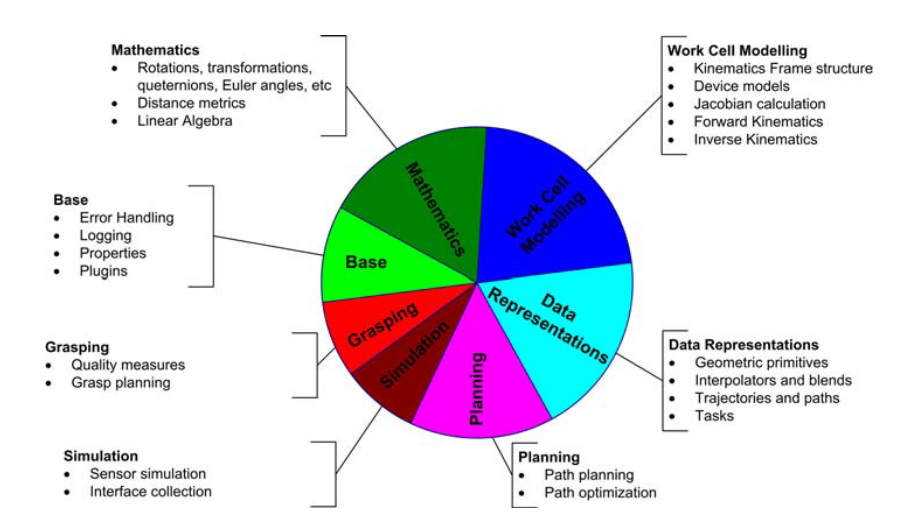
\includegraphics[width=\textwidth]{./graphics/robwork_core_content}
  \footnotetext[1]{Image borrowed from \cite{robwork}}
\end{frame}

% ------------------------------------------------

\begin{frame}
\frametitle{RobWorkStudio}
  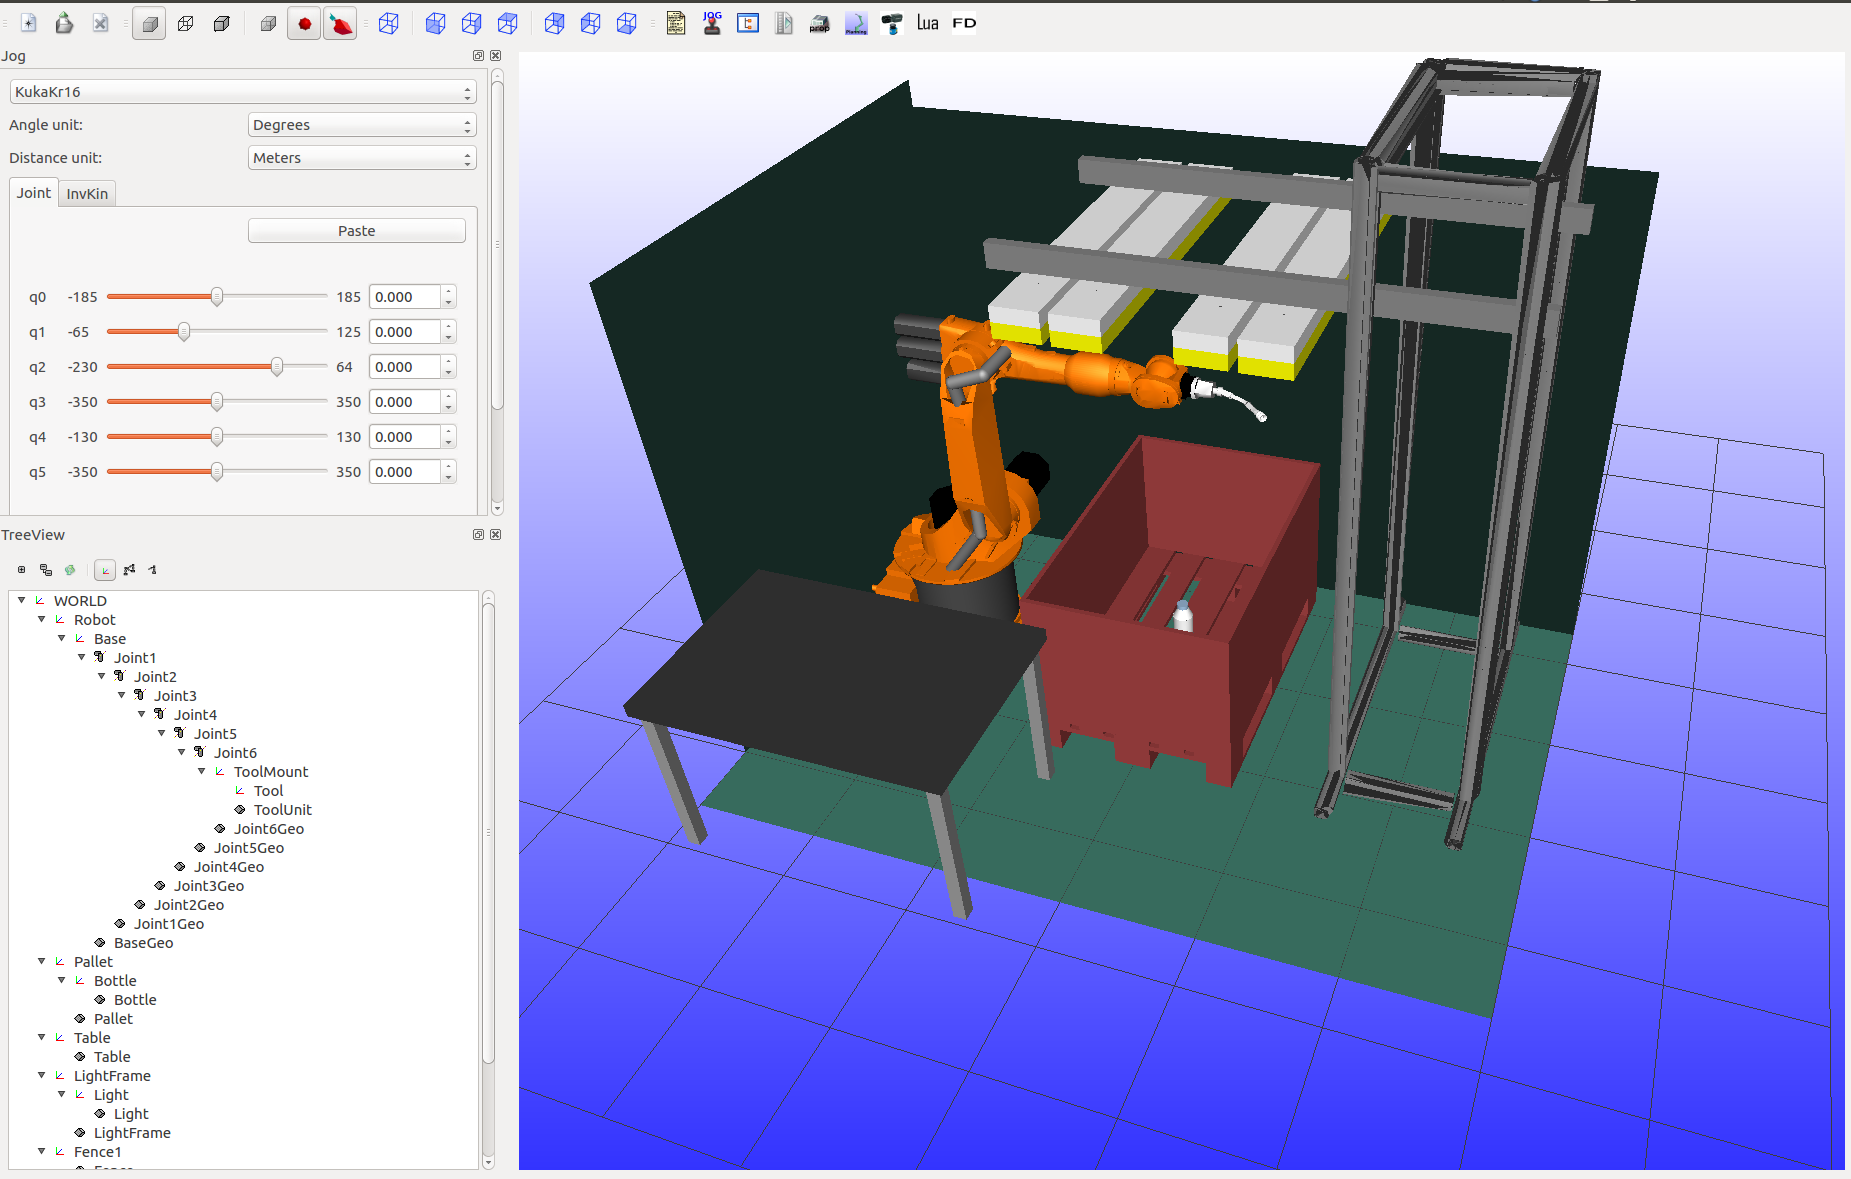
\includegraphics[width=\textwidth]{./graphics/robworkstudio}
\end{frame}

%------------------------------------------------

\section{Exercises for today}

% ------------------------------------------------

\begin{frame}
  \frametitle{Tasks for today}
  \begin{itemize}
  \item Compile and run the HelloRobWork program
  \item Programming Exercise 1.1 and 1.2
  \item Get familiar with RobWorkStudio and robot movement
  \item Use the jog plugin to move the robot
  \item Workcell is available on itslearning
    \item Visualize frames in the Tree plugin
    \item Do Programming Exercise 2
  \item Construct a RobWork workcell with a UR robot manipulator
  \item Geometries are from a CAD file
  \item Use datasheet (on itslearning) to get measurements
  \item Download workcell \texttt{UR5WorkCellCut.zip} from itslearning
  \item Edit the \texttt{Device.wc.xml} file
  \end{itemize}
\end{frame}

% ------------------------------------------------

\section{RobWork Workcell Structure}

% ------------------------------------------------

\begin{frame}
  \frametitle{RobWork Workcell Structure}
  \begin{columns}
    \begin{column}{0.75\textwidth}
      \begin{itemize}
      \item A workcell consists of:
        \begin{itemize}
        \item Geometries
        \item Devices
        \item Scene definitions (Frame definitions)
        \item Collision Setup
        \end{itemize}
      \item Each device is structured as a workcell
      \item More information can be found at \url{http://www.robwork.dk/file_formats/workcell/\#}
      \end{itemize}
    \end{column}
    \begin{column}{0.25\textwidth}
      \begin{centering}
        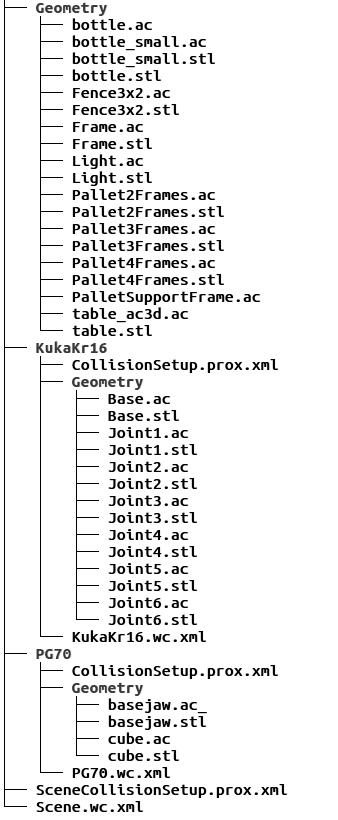
\includegraphics[height=0.75\textheight]{./graphics/workcell_structure}
      \end{centering}
    \end{column}
  \end{columns}
\end{frame}

% ------------------------------------------------



\begin{frame}
  \frametitle{RobWork XML files}
  \begin{itemize}
  \item Frame definitions
    \begin{itemize}
    \item Positions: x, y, z (red, green, blue) in $[m]$
    \item Rotations: RPY ($\theta_z$, $\theta_y$, $\theta_x$) in $[Deg]$
    \item Type: Revolute or prismatic
    \end{itemize}
  \item Joint limits: Have already been set
  \item Drawables
    \begin{itemize}
    \item Graphics for a joint
    \item \texttt{refframe} gives the coordinate frame for the graphics
    \item Pose is relative to \texttt{refframe}
    \item \textbf{WARNING: } The pose of the graphics objects is given in absolute coordinates w.r.t. the robot  
    \end{itemize}
  \end{itemize}
\end{frame}

% ------------------------------------------------

\section{Programming Exercise 2}

\begin{frame}
  \frametitle{Programming Exercise 2}
  \begin{itemize}
  \item Guide to the first two joints.
    \item Based on slides by Lars Carøe Sørensen
  \end{itemize}
\end{frame}

% ------------------------------------------------

\begin{frame}
  \frametitle{Programming Exercise 2}
  \begin{centering}
    \begin{figure}
    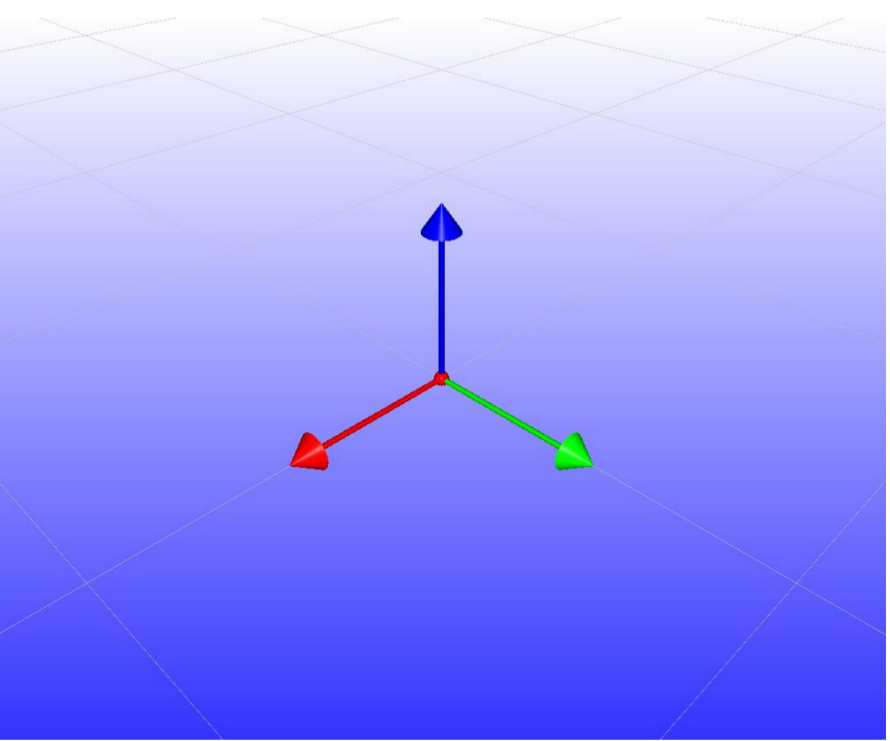
\includegraphics[height=0.6\textheight]{./graphics/ex33_1}
    \caption{World/Robot/Base frame}
    \end{figure}
    \end{centering}
\end{frame}


% ------------------------------------------------

\begin{frame}
  \frametitle{Programming Exercise 2}
  \begin{centering}
    \begin{figure}
    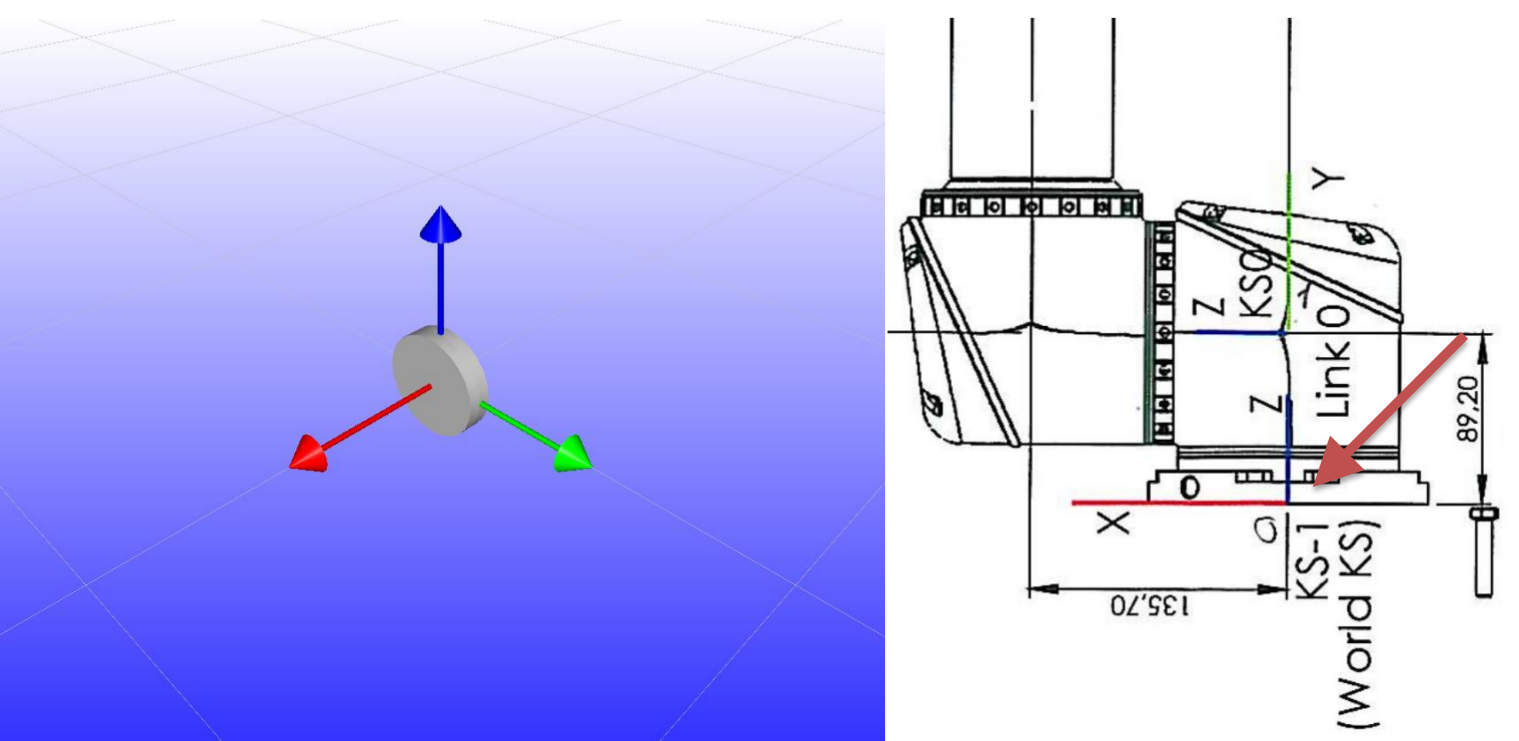
\includegraphics[height=0.6\textheight]{./graphics/ex33_2}
    \caption{Insert robotFlange and base (all pos and rot zero)}
    \end{figure}
    \end{centering}
  \end{frame}
  
% ------------------------------------------------

\begin{frame}
  \frametitle{Programming Exercise 2}
  \begin{centering}
    \begin{figure}
    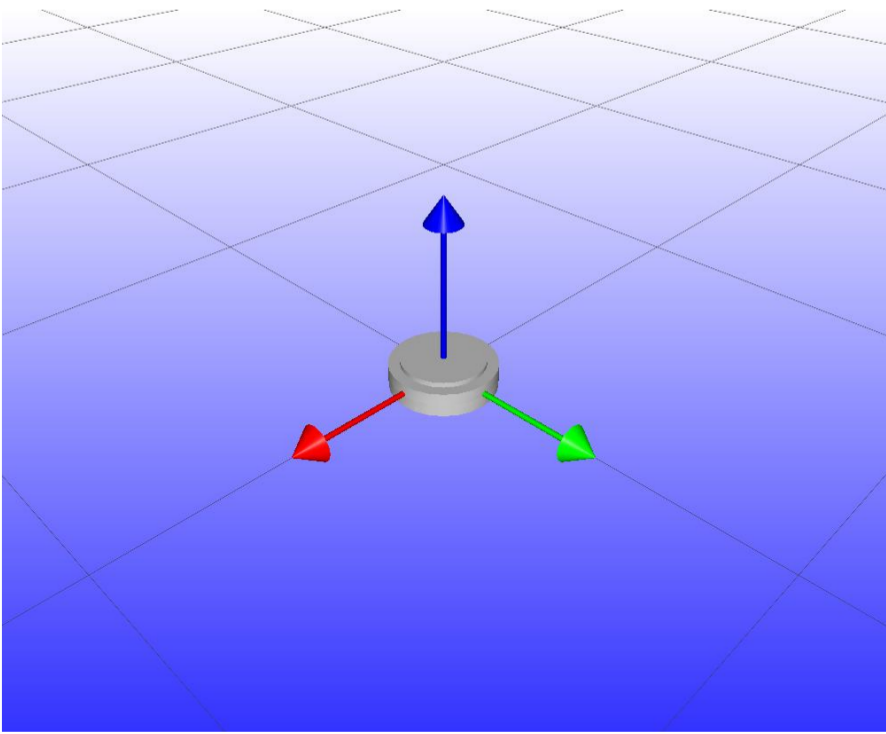
\includegraphics[height=0.6\textheight]{./graphics/ex33_3}
    \caption{Drawable: rotate $90^{\circ}$ about $y$ ($P = 90^{\circ}$)}
    \end{figure}
    \end{centering}
\end{frame}

% ------------------------------------------------

\begin{frame}
  \frametitle{Programming Exercise 2}
  \begin{itemize}
  \item Base and robotFlange in place. XML is:
    \item \texttt{<Drawable name="flangeGeo" refframe="Base">} \newline
      \texttt{<RPY> 0 90 0</RPY> <Pos> 0 0 0</Pos>} \newline
      \texttt{<Polytope file="geometry/robotFlange" />}\newline
      \texttt{</Drawable>}\newline
      \texttt{<Drawable name="baseGeo" refframe="Base">}\newline
      \texttt{<RPY> 0 90 0</RPY> <Pos> 0 0 0</Pos>} \newline
      \texttt{<Polytope file="geometry/base" />} \newline
      \texttt{</Drawable>} 
    \end{itemize}
\end{frame}

% ------------------------------------------------

\begin{frame}
  \frametitle{Programming Exercise 2}
  \begin{centering}
    \begin{figure}
    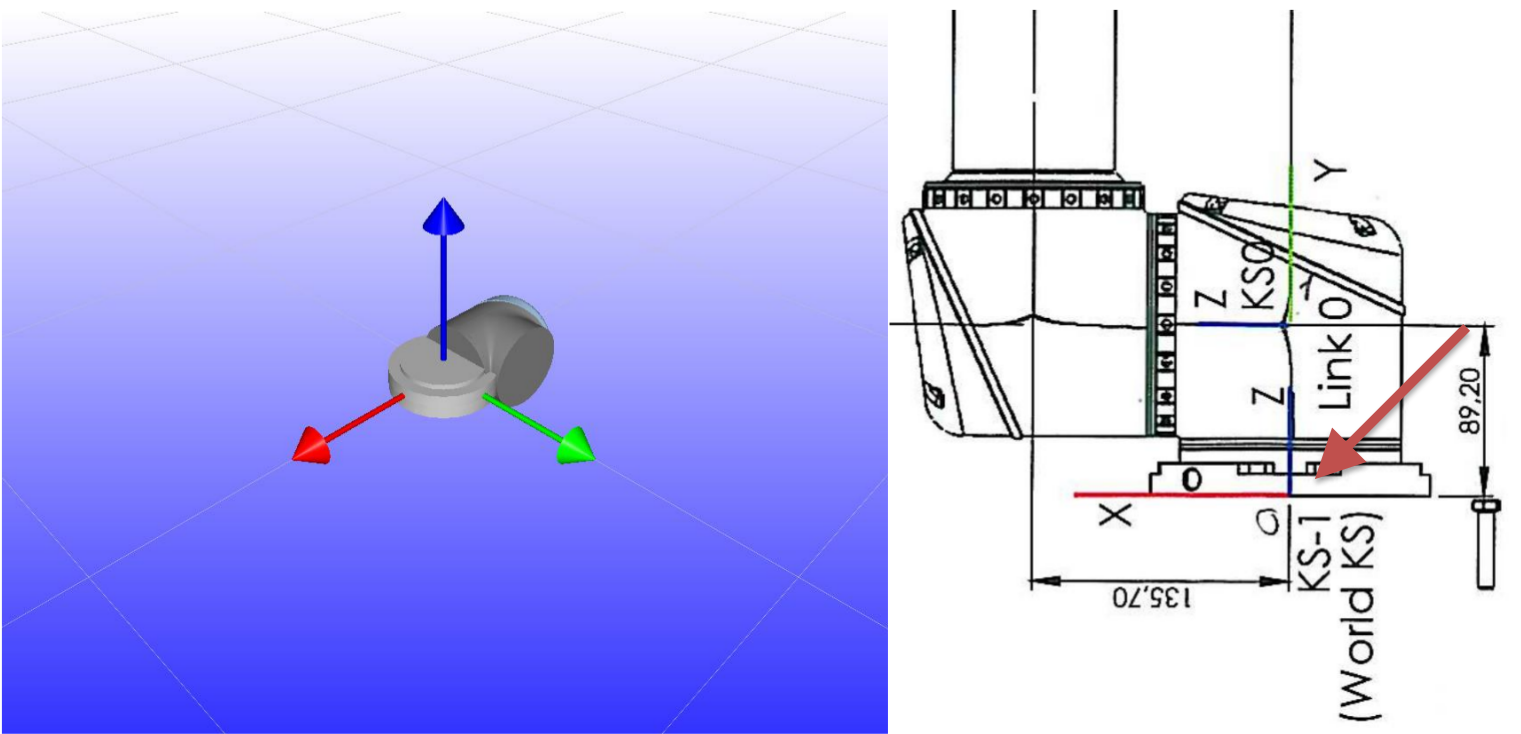
\includegraphics[height=0.6\textheight]{./graphics/ex33_4}
    \caption{Insert Joint0 (all pos and rot zero)}
    \end{figure}
    \end{centering}
  \end{frame}
  
% ------------------------------------------------

\begin{frame}
  \frametitle{Programming Exercise 2}
  \begin{centering}
    \begin{figure}
    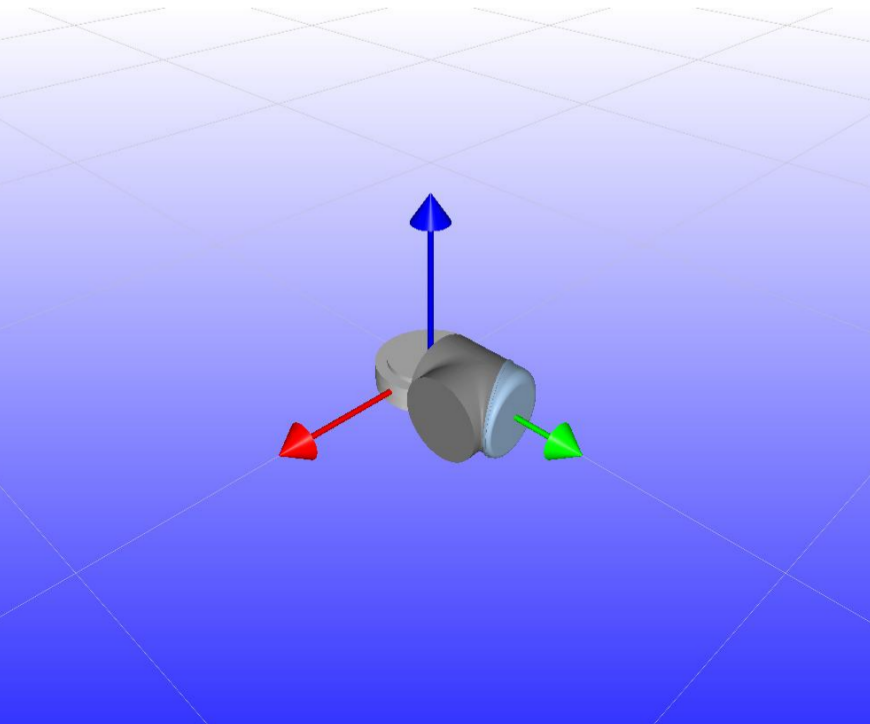
\includegraphics[height=0.6\textheight]{./graphics/ex33_5}
    \caption{Drawable0: rotate $270^{\circ}$ around $z$ ($R=270^{\circ}$)}
    \end{figure}
    \end{centering}
  \end{frame}
  
% ------------------------------------------------

\begin{frame}
  \frametitle{Programming Exercise 2}
  \begin{centering}
    \begin{figure}
    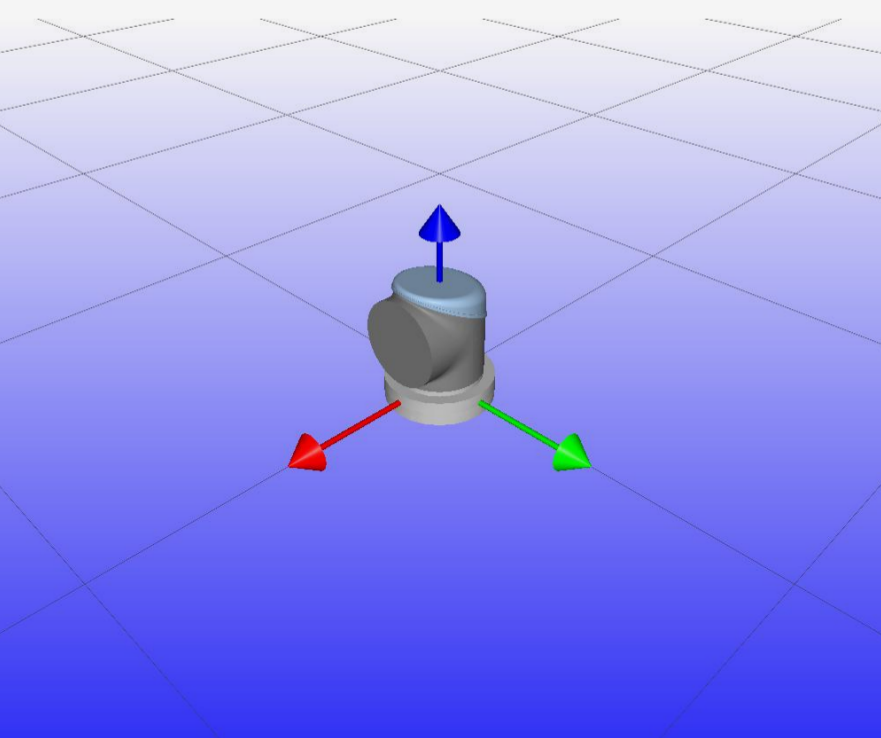
\includegraphics[height=0.6\textheight]{./graphics/ex33_6}
    \caption{Drawable0: rotate $90^{\circ}$ around $y$ ($P=90^{\circ}$)}
    \end{figure}
    \end{centering}
  \end{frame}
  
% ------------------------------------------------

\begin{frame}
  \frametitle{Programming Exercise 2}
  \begin{itemize}
  \item Joint0 in place
    \item \texttt{<Joint name="Joint0" type="Revolute">} \newline
      \texttt{<RPY> 0 0 0 </RPY> <Pos> 0 0 0 </Pos>} \newline
      \texttt{</Joint>} \newline
      \texttt{<Drawable name="Joint0Geo" refframe="Joint0">}\newline
      \texttt{<RPY> 270 90 0 </RPY> <Pos> 0 0 0 </Pos>}\newline
      \texttt{<Polytope file="Geometry/joint0" />}\newline
      \texttt{</Drawable>} \newline
      \texttt{<Q name="Home">0</Q>}
  \end{itemize}
\end{frame}

% ------------------------------------------------

\begin{frame}
  \frametitle{Programming Exercise 2}
  \begin{centering}
    \begin{figure}
    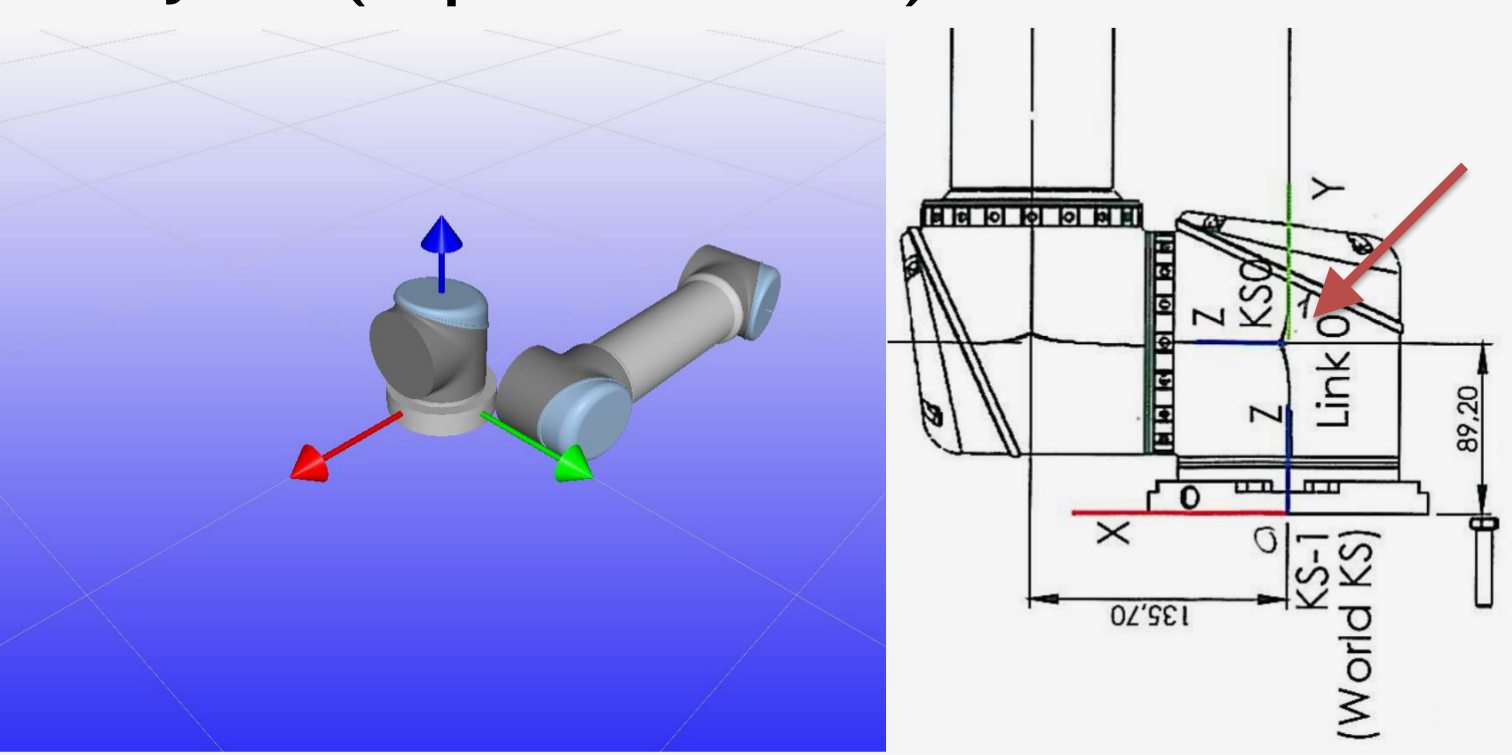
\includegraphics[height=0.6\textheight]{./graphics/ex33_7}
    \caption{Insert Joint1 (all pos and rot zero!)}
    \end{figure}
    \end{centering}
  \end{frame}
  
% ------------------------------------------------

\begin{frame}
  \frametitle{Programming Exercise 2}
  \begin{centering}
    \begin{figure}
    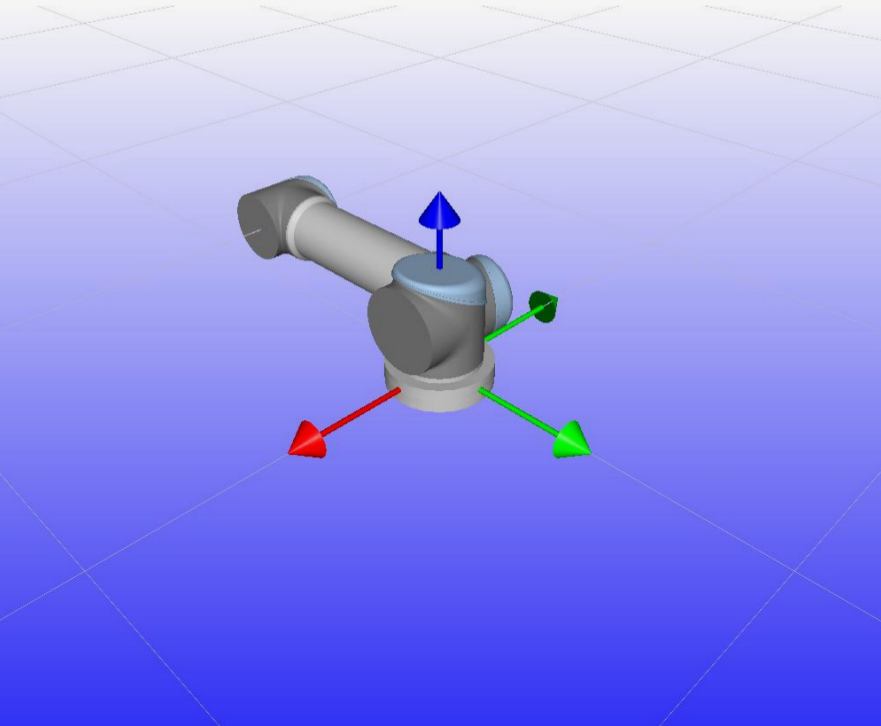
\includegraphics[height=0.6\textheight]{./graphics/ex33_8}
    \caption{Joint1: rotate frame ($R=90^{\circ}$)}
    \end{figure}
    \end{centering}
  \end{frame}
  
% ------------------------------------------------

\begin{frame}
  \frametitle{Programming Exercise 2}
  \begin{centering}
    \begin{figure}
    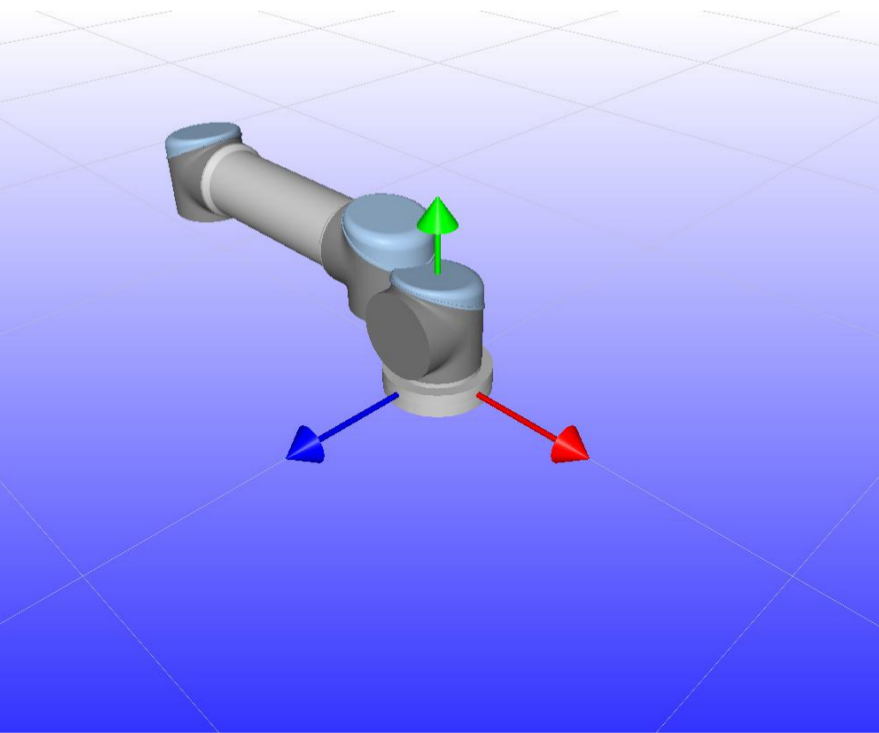
\includegraphics[height=0.6\textheight]{./graphics/ex33_9}
    \caption{Joint1: rotate frame ($Y=90^{\circ}$)}
    \end{figure}
    \end{centering}
  \end{frame}
  
% ------------------------------------------------

\begin{frame}
  \frametitle{Programming Exercise 2}
  \begin{centering}
    \begin{figure}
    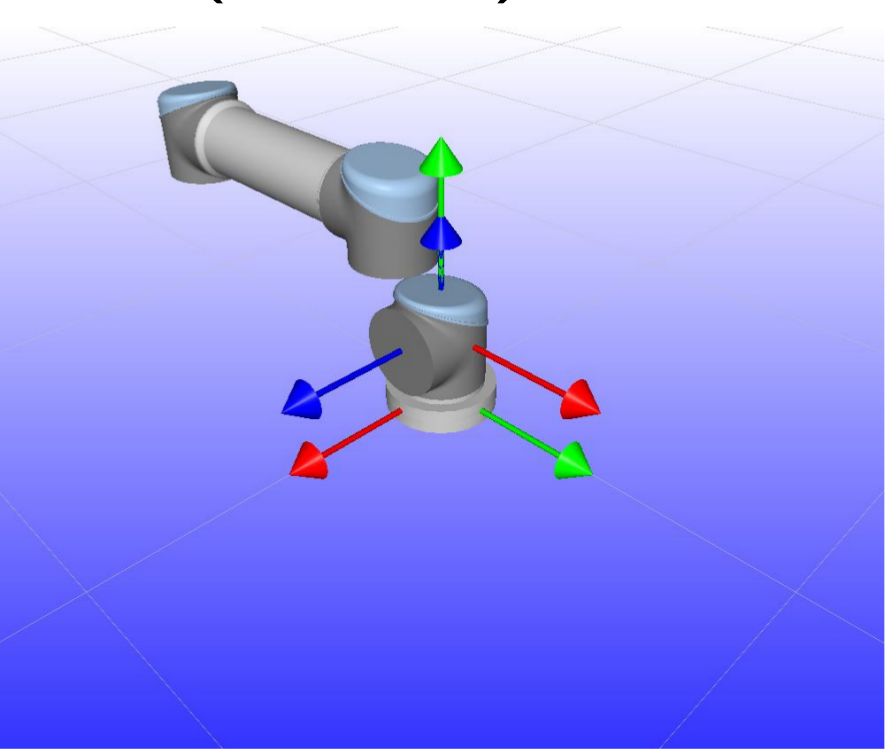
\includegraphics[height=0.6\textheight]{./graphics/ex33_10}
    \caption{Joint1: move frame ($z=0.08920$)}
    \end{figure}
    \end{centering}
  \end{frame}
  
% ------------------------------------------------

\begin{frame}
  \frametitle{Programming Exercise 2}
  \begin{centering}
    \begin{figure}
    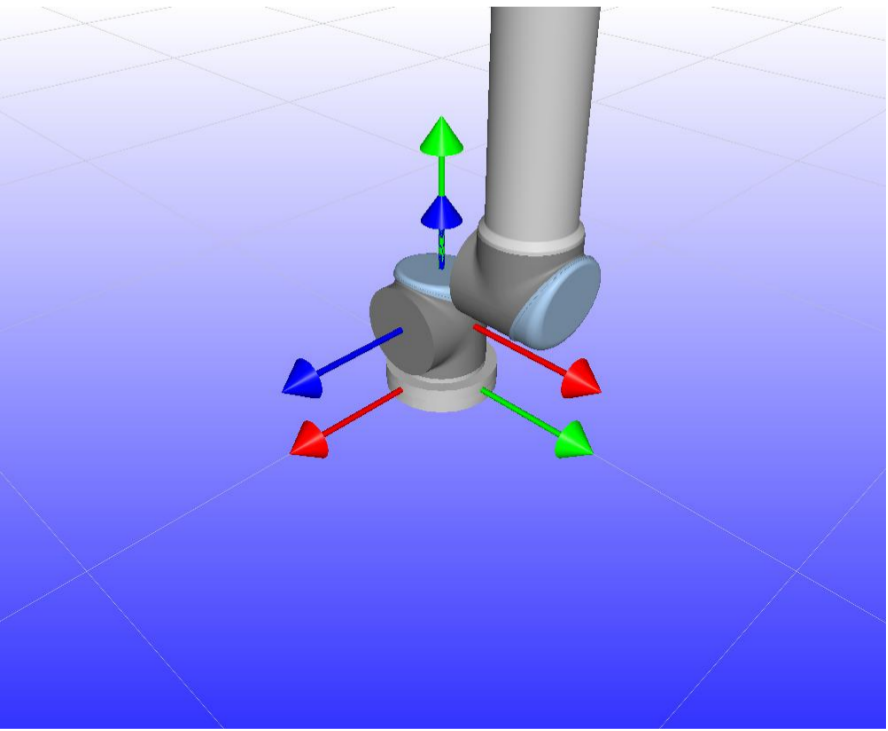
\includegraphics[height=0.6\textheight]{./graphics/ex33_11}
    \caption{Drawable1: rotate drawing ($R=270^{\circ}$)}
    \end{figure}
    \end{centering}
  \end{frame}
  
% ------------------------------------------------

\begin{frame}
  \frametitle{Programming Exercise 2}
  \begin{centering}
    \begin{figure}
    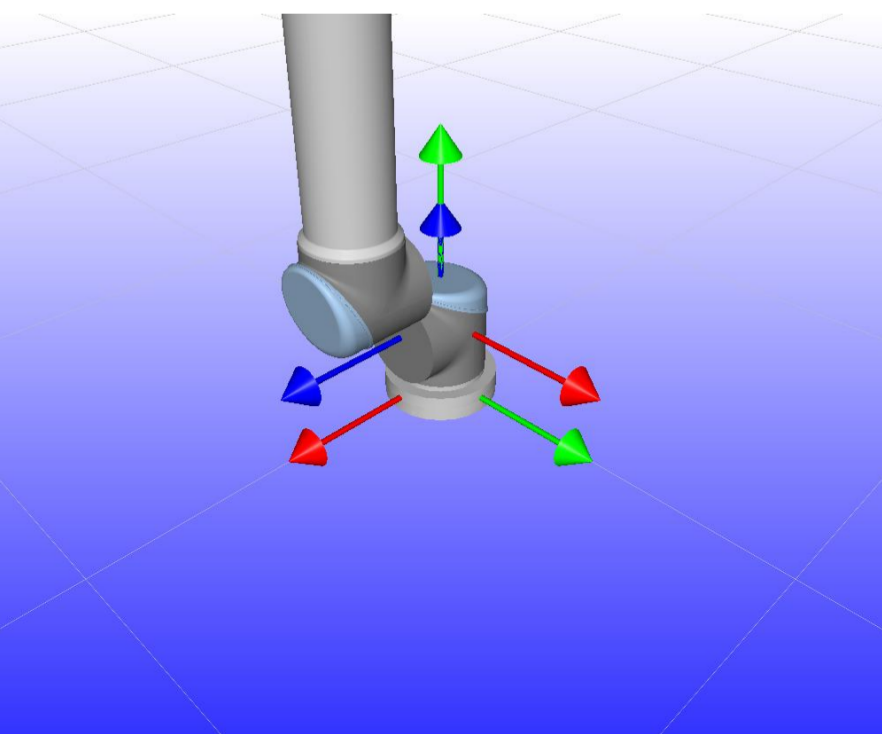
\includegraphics[height=0.6\textheight]{./graphics/ex33_12}
    \caption{Drawable1: rotate drawing ($Y=90^{\circ}$)}
    \end{figure}
    \end{centering}
  \end{frame}
  
% ------------------------------------------------

\begin{frame}
  \frametitle{Programming Exercise 2}
  \begin{centering}
    \begin{figure}
    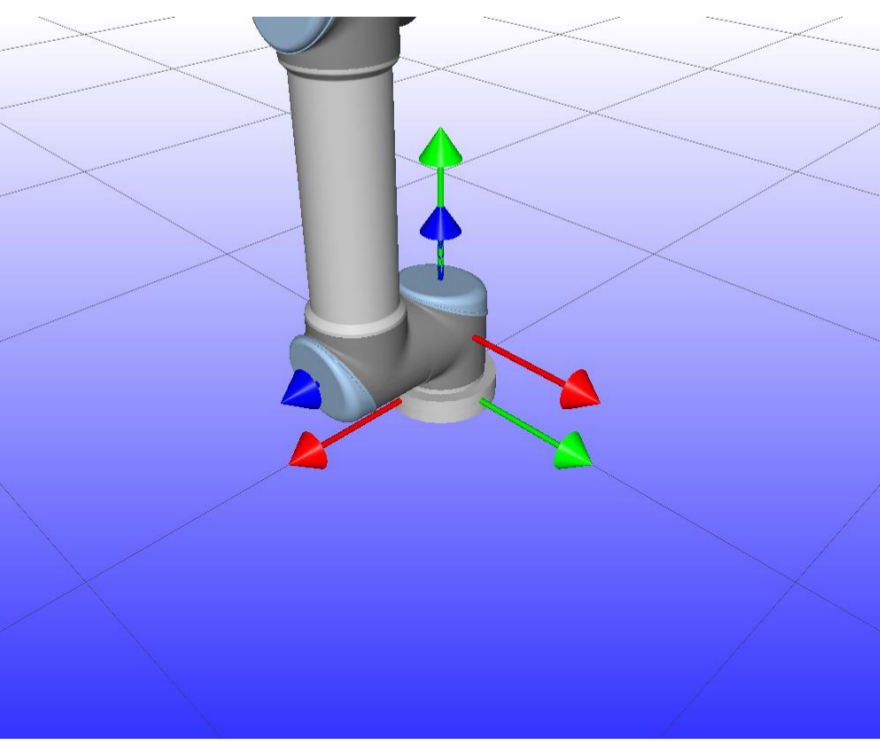
\includegraphics[height=0.6\textheight]{./graphics/ex33_13}
    \caption{Drawable1: move drawing ($y=-0.08920$)}
    \end{figure}
    \end{centering}
  \end{frame}
  
% ------------------------------------------------

\begin{frame}
  \frametitle{Programming Exercise 2}
  \begin{itemize}
  \item Joint1 in place.
    \item \texttt{<Joint name="Joint1" type="Revolute">} \newline
      \texttt{<RPY> 90 0 90 </RPY> <Pos> 0 0 0.0892 </Pos>} \newline
      \texttt{</Joint>} \newline
      \texttt{<Drawable name="Joint1Geo" refframe="Joint1">} \newline
      \texttt{<RPY> 270 0 90 </RPY> <Pos> 0 -0.0892 0</Pos>} \newline
      \texttt{<Polytope file="Geometry/joint1"/>} \newline
      \texttt{</Drawable>} \newline
      \texttt{<Q name="Home">0 0</Q>}
  \end{itemize}
\end{frame}

% ------------------------------------------------

\begin{frame}
  \frametitle{Tips}
  \begin{itemize}
  \item Be systematic in your approach. Either: 
    \begin{itemize}
    \item Rotations before positions
    \item Positions before rotations
    \end{itemize}
  \item Remember to make the home Q vector (end of XML) the right size
  \item Use the diagram from the datasheet for:
    \begin{itemize}
    \item Dimensions of the robot
    \item Position/Orientation of frames
    \end{itemize}
  \item { \color{red} There are small misalignments in the drawables. Ignore these! }
  \end{itemize}
\end{frame}

% ------------------------------------------------
\begin{frame}
\frametitle{References}
\footnotesize{
\begin{thebibliography}{99} % Beamer does not support BibTeX so references must be inserted manually as below
\bibitem[Ellekilde, Jorgensen, 2010]{robwork} L. P. Ellekilde and J. A. Jorgensen (2010)
\newblock RobWork: A Flexible Toolbox for Robotics Research and Education
\newblock \emph{ISR 2010 (41st International Symposium on Robotics) and ROBOTIK 2010 (6th German Conference on Robotics)}, 1 -- 7.
\end{thebibliography}
}
\end{frame}

%----------------------------------------------------------------------------------------

\end{document} 
